\renewcommand{\thefootnote}{\fnsymbol{footnote}}

\chapter[Expected utility theory]%
 {Expected utility theory}
\label{ch:L2}

% 3) Reset things so later footnotes go back to 1, 2, 3, …
%\setcounter{footnote}{0}
\renewcommand{\thefootnote}{\arabic{footnote}}

\section{Assumptions on preferences}\label{sec:L2-intro}

We now impose properties on preferences over lotteries and study their behavioural implications. But first, a brief methodological aside on what we are doing. Before discussing properties of \( \succsim \), we should make explicit what the interpretation of \( \succsim \) is. Different methodological stances are possible. Is \( \succsim \) tracking what an individual has in mind? What he would say if asked? How he chose in the past?

Under \textit{revealed preference theory}, we interpret \( \succsim \) as a description of how an individual \textbf{chooses}. Therefore, there is no psychological content to \( \succsim \). Revealed preference theory has been the standard methodological stance in economics for a long time. But why? Wouldn't it be better to develop a theory that exploits psychological insights?

Revealed preference theory is a methodological stance, not a psychological (or, for that matter, a moral) one. The assumption is not that choices are unrelated to psychological motives, but that we abstract from these motives and look for patterns in choices directly. There is a strong advantage in doing so: psychological motives are hard to observe, while choices can be observed easily. The implication is that a choice theory based on revealed preferences is empirically testable: if we observe choices that violate the theory’s assumptions, we can reject it. Therefore, revealed preference theory is \textbf{not} a claim about how individuals make choices or about what drives them. On the contrary, it is deliberately silent about these issues.\footnote{If you are interested, see \citet{thomaDefenceRevealedPreference2021} for a discussion of the current status of revealed preference theory and \citet{moscatiPsychologicalNarrativesDecision2025} for the role of psychological narratives in choice theory.} This is often misunderstood: there is a plethora of critics claiming that economics views individuals as cold robots.\footnote{By the way, if you read Asimov’s books you know that robots are not cold at all!}

Such critics mostly come from behavioural economics, a field that aims to incorporate psychological insights into economic models.\footnote{See \citet{spieglerCuriousCultureEconomic2024a} for an account of the motivations of the founding fathers of behavioural economics.} Is it therefore impossible to do behavioural economics within the revealed-preference framework? Not at all. Good behavioural theories do what the name suggests: they characterise the \emph{behavioural} content of a theory, so that we, as economists, can understand how individuals behave. Two behavioural theories with different psychological content but that are observationally equivalent—i.e., they make the same predictions about choices—have the same economic implications.\footnote{There is a huge debate on this topic. Among many, I suggest reading \citet{gulCaseMindlessEconomics2008} and the reply by \citet{camererCaseMindfulEconomics2008}. A more recent discussion is \citet{spieglerBehavioralEconomicsAtheoretical2019}.}

\begin{techremark}
	An interesting case study is \cite{masatliogluBehavioralAnalysisStochastic2016}, where the authors show that the famous model by \cite{koszegiReferencedependentRiskAttitudes2007} is behaviourally equivalent to the intersection of rank-dependent utility and quadratic utility—two older models—despite having a different psychological interpretation. Another example that is quite relevant today is in \cite{eliazCanAnticipatoryFeelings2006}.
\end{techremark}

In what follows, you can have in mind the interpretation of \( \succsim \) that you prefer, but keep in mind that assumptions may have different flavours under different interpretations. Recall that we want to find properties that single out expected utility preferences in Equation~\eqref{eq:eu0}. Therefore, it might be worthwhile to first understand some implications of having expected utility preferences.

Having expected utility preferences over lotteries implies that indifference curves on the simplex are straight lines. That is, say that if \( p \sim q \), then, for any \( \alpha \in (0,1) \), it holds that \( \alpha p + (1-\alpha) q \sim p \), as illustrated in Figure~\ref{fig:simplex-ind}.

\begin{figure}[H]
	\centering
	% \usetikzlibrary{calc} % <-- enable if you keep the ($(P)!t!(Q)$) syntax
	\begin{tikzpicture}[scale=1]
		% small filled dot style
		\tikzset{dot/.style={circle,fill,inner sep=1.4pt}}

		%--- simplex vertices --------------------------------------------------------
		\coordinate (A) at (0,0);
		\coordinate (B) at (6,0);
		\coordinate (C) at (3,5.196); % = (sqrt(3)/2)*6

		\draw[thick] (A)--(B)--(C)--cycle;

		% vertex labels = degenerate lotteries
		\node[dot] at (A) {};
		\node[below,align=center] at (A) {$x$ \\ {\scriptsize $(1,0,0)$}};
		\node[dot] at (B) {};
		\node[below,align=center] at (B) {$y$ \\ {\scriptsize $(0,1,0)$}};
		\node[dot] at (C) {};
		\node[above,align=center] at (C) {{\scriptsize $(0,0,1)$}\\[-2pt] $z$};

		%--- two interior lotteries p and q -----------------------------------------
		\coordinate (P) at (1.7,1.35);
		\coordinate (Q) at (4.2,1.15);

		\node[dot] at (P) {};
		\node[above left=2pt] at (P) {$p$};

		\node[dot] at (Q) {};
		\node[above right=2pt] at (Q) {$q$};

		% segment of mixtures r_λ = λ p + (1-λ) q  (indifference set if p ~ q)
		\draw[very thick] (P)--(Q);

		% an example interior mixture point on the segment
		\coordinate (R) at ($(P)!0.42!(Q)$); % requires calc library
		\node[below=3pt] at (R) {$\alpha p+(1-\alpha)q$};

	\end{tikzpicture}
	\caption{If \( p \sim q \), then any mixture of \( p \) and \( q \) is also indifferent to \( p \) and \( q \).}
	\label{fig:simplex-ind}
\end{figure}

Let's show this formally. Assume that \( p \sim q \). Then, by the definition of expected utility, we have

\[
	\sum_{x\in X} p(x)u(x) = \sum_{x\in X} q(x)u(x).
\]

Applying expected utility again, for any \( \alpha \in (0,1) \), the utility of the lottery \( \alpha p + (1-\alpha) q \) is

\begin{align*}
	\sum_{x\in X} \big(\alpha p(x) + (1-\alpha) q(x)\big) u(x)
	 & = \sum_{x\in X} \alpha p(x) u(x) + \sum_{x\in X} (1-\alpha) q(x) u(x) \\
	 & = \alpha \sum_{x\in X} p(x) u(x) + (1-\alpha) \sum_{x\in X} q(x) u(x) \\
	 & = \alpha \sum_{x\in X} q(x) u(x) + (1-\alpha) \sum_{x\in X} q(x) u(x) \\
	 & = \sum_{x\in X} q(x) u(x).
\end{align*}

Indifference curves are also parallel; you are asked to show this in Exercise~\ref{ex:parallel-lines}. Of course, the fact that indifference curves are straight lines is related to the linearity of expected utility, which in turn follows from a specific axiom, as we will see shortly.

Let's now turn to the properties of \( \succsim \) we will consider. First, we assume that preferences form a \textbf{weak order}.

\begin{axiom}\label{ax:wo}
	\labelname{axn:wo}{Weak order} (\textbf{Weak order}) Preferences \(\succsim\) are complete and transitive.
\end{axiom}

Recall that preferences are \textbf{complete} if, for any two lotteries \(p,q\), either \(p\succsim q\) or \(q\succsim p\), or both. They are \textbf{transitive} if, for any three lotteries \(p,q,r\), whenever \(p\succsim q\) and \(q\succsim r\), then \(p\succsim r\).

\begin{techremark}
	Sometimes \usename{axn:wo} is referred to as \textbf{rationality} of preferences (see e.g. \citet[p.~6]{mas-colellMicroeconomicTheory1995}). However, I think this is an unfortunate name. It suggests that it is \enquote{irrational} to violate \usename{axn:wo}, but there are reasons why people might have intransitive or incomplete preferences (can you think of any?).
\end{techremark}

\usename{axn:wo} is a necessary condition for having any utility representation (see \citet[p.~9]{mas-colellMicroeconomicTheory1995}). It is not the core assumption of expected utility theory, but rather one shared by most theories of choice.

\begin{axiom}\label{ax:continuity}
	\labelname{axn:continuity}{Continuity} (\textbf{Continuity}) For any three lotteries \(p,q,r\), if \(p\succ q\succ r\), then there exist \(\alpha,\beta\in(0,1)\) such that \(\alpha p+(1-\alpha)r\succ q\succ \beta p+(1-\beta)r\).
\end{axiom}

\usename{axn:continuity} says that there is no lottery \( p \) so good that, for \( q \succ r \), a small probability \( \beta \) of \( p \) and a large probability \( 1-\beta \) of \( r \) is always better than \( q \). Similarly, there is no gamble \(r\) so bad that, for \( p \succ q \), a large probability \(\alpha \) of \(p\) and a small probability \(1-\alpha\) of \(r\) is always worse than \(q\). In essence, this axiom implies that preferences do not have \enquote{jumps} when probabilities change slightly—i.e., that preferences are \emph{continuous} in probabilities. \usename{axn:continuity} allows us to obtain a continuous utility representation of preferences (see \citet[p.~47]{mas-colellMicroeconomicTheory1995}), but again, it is not the core assumption of expected utility theory—the next one is.

\begin{axiom}
	\labelname{axn:independence}{Independence} (\textbf{Independence}) For any three lotteries \(p,q,r\) and for any \(\alpha\in(0,1)\), we have \( p \succsim q \) if and only if \(\alpha p+(1-\alpha)r\succsim \alpha q+(1-\alpha)r\).
\end{axiom}

In words, \usename{axn:independence} says that if \(p\) is preferred to \(q\), then mixing both lotteries with any third lottery \(r\), using the same probability \(1-\alpha\), does not change their ranking. One way to justify \usename{axn:independence} is as follows. Suppose \(p \succsim q\). Now consider two compound lotteries obtained by tossing a coin: the first yields \(p\) if the coin shows heads and \(r\) otherwise; the second yields \(q\) if the coin shows heads and \(r\) otherwise. Ex ante, one might reason that what happens if the coin shows tails is the same in both compound lotteries, so that part should not matter—while if the coin shows heads, \(p\) is preferred to \(q\). Therefore, the first compound lottery should be preferred to the second.

This argument relies on the meaning of the mixing operation within the set of lotteries. By contrast, consider the case of mixing foods. One might prefer pasta to cake, yet mixing both with whipped cream could make the cake better than the pasta.\footnote{Feel no shame if you are unconvinced by this example.} You are asked in Exercise~\ref{ex:indlin} to elaborate on the relation between \usename{axn:independence} and the linearity of indifference curves.

Before stating Theorem~\ref{thm:eu} in the next section, we need to prove a preliminary result. Lemma~\ref{lem:max} establishes that, under the assumptions introduced so far, there exist two lotteries that are the best and the worst possible ones.

\begin{lemma}\label{lem:max}
	Let \( \succsim \) satisfy \usename{axn:wo} and \usename{axn:independence}. Then there exist two lotteries \( \overline p \) and \( \underline p \) such that
	\[
		\overline p \succsim p \succsim \underline p \quad \text{for all } p .
	\]
\end{lemma}

\begin{proof}
	The proof proceeds in two steps.

	\paragraph{Step 1.} By \usename{axn:wo}, the restriction of \( \succsim \) to the set of degenerate lotteries \(\{\delta_x \in \Delta(X): \delta_x(x) = 1\}\) is a complete and transitive order on a finite set. Hence there exist outcomes \(x^\ast, x_\ast\) such that
	\[
		\delta_{x^\ast} \succsim \delta_x \succsim \delta_{x_\ast}
		\qquad \text{for all } x.
	\]
	Fix \( \overline p := \delta_{x^\ast} \) and \( \underline p := \delta_{x_\ast} \).

	\paragraph{Step 2.} For any lottery \( p \), let \(\mathrm{supp}(p) = \{x \in X : p(x) > 0\}\) and denote its size by \(|\mathrm{supp}(p)|\). We prove by induction on \(k := |\mathrm{supp}(p)|\) that
	\[
		\overline p \succsim p \succsim \underline p.
	\]

	\emph{Base case.} If \(k = 1\), then \(p = \delta_x\) for some \(x\), and the claim follows from \textbf{Step 1}.

	\emph{Inductive step.} Assume the statement holds for all lotteries whose support size is at most \(k-1\). Let \(p\) have support size \(k \ge 2\). Pick any \(x \in \mathrm{supp}(p)\) and write
	\[
		p = \alpha\,\delta_x + (1-\alpha)\,q,
		\qquad \alpha := p(x) \in (0,1),
	\]
	where \(q\) is the renormalized remainder, defined by
	\[
		q(y) =
		\begin{cases}
			\dfrac{p(y)}{1-\alpha} & \text{if } y \neq x, \\[6pt]
			0                      & \text{if } y = x.
		\end{cases}
	\]
	Then \(q \in \Delta(X)\) and \(|\mathrm{supp}(q)| \le k-1\).

	By the inductive hypothesis, \(\overline p \succsim q\); and by \textbf{Step 1}, \(\overline p \succsim \delta_x\). We apply \usename{axn:independence} twice.

	\smallskip
	From \(\overline p \succsim q\), mix with \(\overline p\):
	\[
		\overline p = (1-\alpha)\,\overline p + \alpha\,\overline p
		~\succsim~ (1-\alpha)\,q + \alpha\,\overline p
		= \alpha\,\overline p + (1-\alpha)\,q.
	\]
	From \(\overline p \succsim \delta_x\), mix with \( q\):
	\[
		\alpha\,\overline p + (1-\alpha)\,q
		~\succsim~ \alpha\,\delta_x + (1-\alpha)\,q
		= p.
	\]
	By transitivity,
	\[
		\overline p \succsim p.
	\]

	A symmetric argument yields \(p \succsim \underline p\). Indeed, by the inductive hypothesis \(q \succsim \underline p\) and by \textbf{Step 1} \(\delta_x \succsim \underline p\). Using \usename{axn:independence} with the same reasoning gives
	\[
		p = \alpha\,\delta_x + (1-\alpha)\,q
		~\succsim~ \alpha\,\underline p + (1-\alpha)\,q
		~\succsim~ \underline p.
	\]

	Therefore, \(\overline p \succsim p \succsim \underline p\) for all lotteries with support size \(k\), completing the induction. The fixed degenerate lotteries \(\overline p = \delta_{x^\ast}\) and \(\underline p = \delta_{x_\ast}\) bound every \(p\), as claimed.
\end{proof}


\section{Expected utility representation}

We are ready to state and prove the theorem relating the properties of preferences over lotteries to the expected utility functional form.

\begin{theorem}\label{thm:eu}
	Preferences over lotteries \(\succsim\) satisfy \usename{axn:wo}, \usename{axn:continuity}, and \usename{axn:independence} if and only if there exists a utility function \(u \colon X \to \mathbb{R}\) such that
	\begin{equation}
		p \succsim q \ \text{if and only if}\ \sum_{x\in X} p(x)\,u(x) \ge \sum_{x\in X} q(x)\,u(x) \quad \text{for all } p,q .
	\end{equation}
\end{theorem}

The proof essentially follows \citet[pp.~176–178]{mas-colellMicroeconomicTheory1995}, complemented by intuition and figures.

\begin{proof}
	We proceed by steps.

	\paragraph{Step 1.} If \( p \succsim q \), then \( p \succsim \alpha p + (1-\alpha) q \succsim q \) for any \( \alpha \in (0,1) \).

	The intuition behind this step is simple: if \( p \) is better than \( q \), then any mixture of the two is worse than \( p \) and better than \( q \). Figure~\ref{fig:step1} illustrates the idea.

	\begin{figure}[H]
		\centering
		\tikzset{every picture/.style={line width=0.75pt}} %set default line width to 0.75pt        

		\begin{tikzpicture}[x=0.65pt,y=0.65pt,yscale=-1,xscale=1]
			%uncomment if require: \path (0,412); %set diagram left start at 0, and has height of 412

			%Shape: Triangle [id:dp7624353544488017] 
			\draw   (292.33,43.07) -- (474.67,369.07) -- (110,369.07) -- cycle ;
			%Straight Lines [id:da31966546289590647] 
			\draw  [dash pattern={on 4.5pt off 4.5pt}]  (262,220.92) -- (398.67,316.25) ;
			%Shape: Circle [id:dp6804955961429688] 
			\draw  [fill={rgb, 255:red, 0; green, 0; blue, 0 }  ,fill opacity=1 ] (396.25,316.25) .. controls (396.25,314.92) and (397.33,313.83) .. (398.67,313.83) .. controls (400,313.83) and (401.08,314.92) .. (401.08,316.25) .. controls (401.08,317.58) and (400,318.67) .. (398.67,318.67) .. controls (397.33,318.67) and (396.25,317.58) .. (396.25,316.25) -- cycle ;
			%Shape: Circle [id:dp44734973339031014] 
			\draw  [fill={rgb, 255:red, 0; green, 0; blue, 0 }  ,fill opacity=1 ] (259.58,220.92) .. controls (259.58,219.58) and (260.67,218.5) .. (262,218.5) .. controls (263.33,218.5) and (264.42,219.58) .. (264.42,220.92) .. controls (264.42,222.25) and (263.33,223.33) .. (262,223.33) .. controls (260.67,223.33) and (259.58,222.25) .. (259.58,220.92) -- cycle ;
			%Curve Lines [id:da39390655998084656] 
			\draw    (330.33,268.58) .. controls (378.93,256.92) and (391.95,237.98) .. (405.07,206.2) ;
			\draw [shift={(405.67,204.74)}, rotate = 112.2] [color={rgb, 255:red, 0; green, 0; blue, 0 }  ][line width=0.75]    (10.93,-3.29) .. controls (6.95,-1.4) and (3.31,-0.3) .. (0,0) .. controls (3.31,0.3) and (6.95,1.4) .. (10.93,3.29)   ;
			%Shape: Circle [id:dp4485716510591613] 
			\draw  [fill={rgb, 255:red, 0; green, 0; blue, 0 }  ,fill opacity=1 ] (327.92,268.58) .. controls (327.92,267.25) and (329,266.17) .. (330.33,266.17) .. controls (331.67,266.17) and (332.75,267.25) .. (332.75,268.58) .. controls (332.75,269.92) and (331.67,271) .. (330.33,271) .. controls (329,271) and (327.92,269.92) .. (327.92,268.58) -- cycle ;

			% Text Node
			\draw (392.67,176.4) node [anchor=north west][inner sep=0.75pt]    {$\alpha p +( 1-\alpha ) q\ $};
			% Text Node
			\draw (254,192.4) node [anchor=north west][inner sep=0.75pt]    {$p$};
			% Text Node
			\draw (406,306.4) node [anchor=north west][inner sep=0.75pt]    {$q$};


		\end{tikzpicture}
		\caption{Step 1.}
		\label{fig:step1}
	\end{figure}

	This follows from \usename{axn:independence}.

	\begin{equation}\label{eq:comp1}
		p \succsim q \ \implies\ (1-\alpha)\,p + \alpha\,p \succsim (1-\alpha)\,q + \alpha\,p \ \implies\ p \succsim \alpha p + (1-\alpha) q.
	\end{equation}

	\begin{equation}\label{eq:comp2}
		p \succsim q \ \implies\ \alpha p + (1-\alpha) q \succsim \alpha q + (1-\alpha) q \ \implies\ \alpha p + (1-\alpha) q \succsim q.
	\end{equation}

	The conclusion follows from Equations~\eqref{eq:comp1} and~\eqref{eq:comp2}.

	\paragraph{Step 2.} \(\beta > \alpha\) if and only if \( \beta \overline{p} + (1-\beta)\,\underline{p} \succ \alpha \overline{p} + (1-\alpha)\,\underline{p} \), where \( \overline{p} \) and \( \underline{p} \) are the best and worst lotteries identified in Lemma~\ref{lem:max}.

	The idea of this step is as follows. From \textbf{Step 1}, we know that a mixture of \( p \) and \( q \), where \( p \succsim q \), is worse than \( p \) and better than \( q \). Now, since \( \overline{p} \) is the best lottery available, we have \( \overline{p} \succ \alpha \overline{p} + (1-\alpha)\,\underline{p} \). We want to show that \( \beta \overline{p} + (1-\beta)\,\underline{p} \) can be written as a mixture of \( \overline{p} \) and \( \alpha \overline{p} + (1-\alpha)\,\underline{p} \); therefore, by \textbf{Step 1}, it must be preferred to \( \alpha \overline{p} + (1-\alpha)\,\underline{p} \). The idea is illustrated in Figure~\ref{fig:step2}.

	\begin{figure}[H]
		\centering
		\tikzset{every picture/.style={line width=0.75pt}} %set default line width to 0.75pt        
		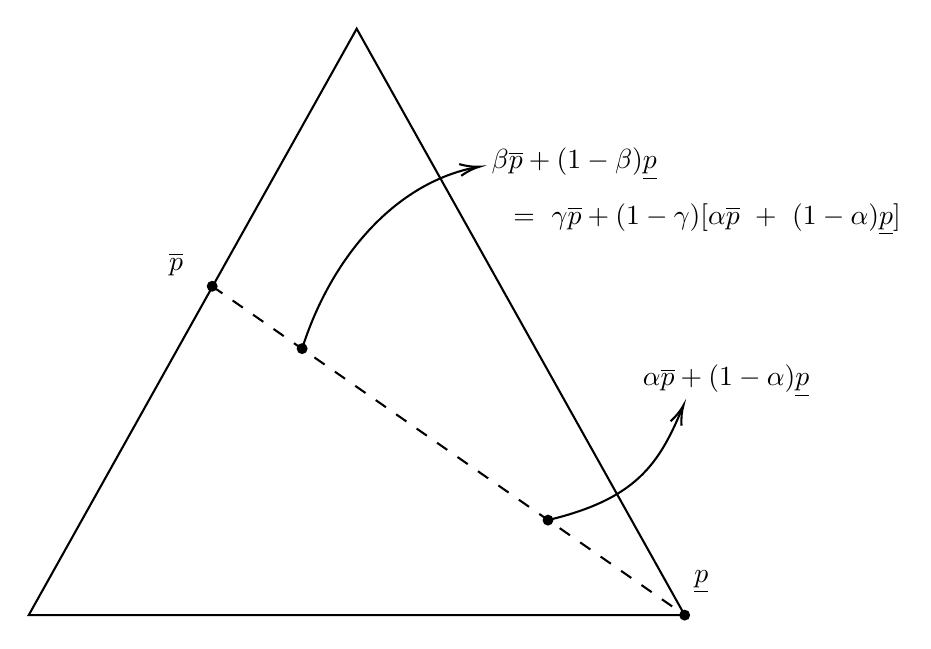
\begin{tikzpicture}[x=0.65pt,y=0.65pt,yscale=-1,xscale=1]
			%uncomment if require: \path (0,376); %set diagram left start at 0, and has height of 376
			%Shape: Triangle [id:dp5718796353912894] 
			\draw   (329.33,23.07) -- (511.67,349.07) -- (147,349.07) -- cycle ;
			%Shape: Circle [id:dp9404346697828574] 
			\draw  [fill={rgb, 255:red, 0; green, 0; blue, 0 }  ,fill opacity=1 ] (509.25,349.07) .. controls (509.25,347.74) and (510.33,346.66) .. (511.67,346.66) .. controls (513,346.66) and (514.08,347.74) .. (514.08,349.07) .. controls (514.08,350.41) and (513,351.49) .. (511.67,351.49) .. controls (510.33,351.49) and (509.25,350.41) .. (509.25,349.07) -- cycle ;
			%Shape: Circle [id:dp21608178484403062] 
			\draw  [fill={rgb, 255:red, 0; green, 0; blue, 0 }  ,fill opacity=1 ] (246.58,166.25) .. controls (246.58,164.92) and (247.67,163.83) .. (249,163.83) .. controls (250.33,163.83) and (251.42,164.92) .. (251.42,166.25) .. controls (251.42,167.58) and (250.33,168.67) .. (249,168.67) .. controls (247.67,168.67) and (246.58,167.58) .. (246.58,166.25) -- cycle ;
			%Straight Lines [id:da0014271293885499414] 
			\draw  [dash pattern={on 4.5pt off 4.5pt}]  (249,166.25) -- (511.67,349.07) ;
			%Shape: Circle [id:dp09512564117547329] 
			\draw  [fill={rgb, 255:red, 0; green, 0; blue, 0 }  ,fill opacity=1 ] (433.25,296.25) .. controls (433.25,294.92) and (434.33,293.83) .. (435.67,293.83) .. controls (437,293.83) and (438.08,294.92) .. (438.08,296.25) .. controls (438.08,297.58) and (437,298.67) .. (435.67,298.67) .. controls (434.33,298.67) and (433.25,297.58) .. (433.25,296.25) -- cycle ;
			%Shape: Circle [id:dp3186545134308967] 
			\draw  [fill={rgb, 255:red, 0; green, 0; blue, 0 }  ,fill opacity=1 ] (296.58,200.92) .. controls (296.58,199.58) and (297.67,198.5) .. (299,198.5) .. controls (300.33,198.5) and (301.42,199.58) .. (301.42,200.92) .. controls (301.42,202.25) and (300.33,203.33) .. (299,203.33) .. controls (297.67,203.33) and (296.58,202.25) .. (296.58,200.92) -- cycle ;
			%Curve Lines [id:da7950025520809244] 
			\draw    (435.67,296.25) .. controls (484.26,284.58) and (497.28,265.65) .. (510.4,233.87) ;
			\draw [shift={(511,232.41)}, rotate = 112.2] [color={rgb, 255:red, 0; green, 0; blue, 0 }  ][line width=0.75]    (10.93,-3.29) .. controls (6.95,-1.4) and (3.31,-0.3) .. (0,0) .. controls (3.31,0.3) and (6.95,1.4) .. (10.93,3.29)   ;
			%Curve Lines [id:da31359625192132545] 
			\draw    (299,200.92) .. controls (314.84,150.91) and (350.28,108.59) .. (396.27,99.99) ;
			\draw [shift={(397.67,99.74)}, rotate = 170.27] [color={rgb, 255:red, 0; green, 0; blue, 0 }  ][line width=0.75]    (10.93,-3.29) .. controls (6.95,-1.4) and (3.31,-0.3) .. (0,0) .. controls (3.31,0.3) and (6.95,1.4) .. (10.93,3.29)   ;

			% Text Node
			\draw (223.33,146.07) node [anchor=north west][inner sep=0.75pt]    {$\overline{p}$};
			% Text Node
			\draw (515.33,322.4) node [anchor=north west][inner sep=0.75pt]    {$\underline{p}$};
			% Text Node
			\draw (486.67,208.4) node [anchor=north west][inner sep=0.75pt]    {$\alpha \overline{p} +( 1-\alpha )\underline{p} \ $};
			% Text Node
			\draw (402.67,87.73) node [anchor=north west][inner sep=0.75pt]    {$\beta \overline{p} +( 1-\beta )\underline{p} \ $};
			% Text Node
			\draw (414.67,118.73) node [anchor=north west][inner sep=0.75pt]    {$=\ \gamma \overline{p} +( 1-\gamma )[ \alpha \overline{p} \ +\ ( 1-\alpha )\underline{p}]$};


		\end{tikzpicture}
		\caption{Step 2.}
		\label{fig:step2}
	\end{figure}

	We want to express \( \beta \overline{p} + (1-\beta)\,\underline{p} \) as a mixture of \( \overline{p} \) and \( \alpha \overline{p} + (1-\alpha)\,\underline{p} \). That is, we look for some \( \gamma \in (0,1) \) such that
	\[
		\beta \overline{p} + (1-\beta)\,\underline{p}
		= \gamma \overline{p} + (1-\gamma)\bigl[\alpha \overline{p} + (1-\alpha)\,\underline{p}\bigr].
	\]
	A short calculation shows that \( \gamma = \dfrac{\beta - \alpha}{1 - \alpha} \). By \textbf{Step 1} we know that \( \overline{p} \succ \alpha \overline{p} + (1-\alpha)\,\underline{p} \); therefore,
	\[
		\gamma \overline{p} + (1-\gamma)\bigl[\alpha \overline{p} + (1-\alpha)\,\underline{p}\bigr]
		\succ \alpha \overline{p} + (1-\alpha)\,\underline{p}.
	\]
	Since \( \beta \overline{p} + (1-\beta)\,\underline{p}
	= \gamma \overline{p} + (1-\gamma)\bigl[\alpha \overline{p} + (1-\alpha)\,\underline{p}\bigr] \), the conclusion follows.

	Up to this point we have proved that if \( \beta > \alpha \), then \( \beta \overline{p} + (1-\beta)\,\underline{p} \succ \alpha \overline{p} + (1-\alpha)\,\underline{p} \). But the statement says \enquote{if and only if}, so we must also show the converse: if \( \alpha \ge \beta \), then it cannot be that \( \beta \overline{p} + (1-\beta)\,\underline{p} \succ \alpha \overline{p} + (1-\alpha)\,\underline{p} \). When \( \beta = \alpha \), the two lotteries coincide and are therefore indifferent. The relevant case is \( \alpha > \beta \). By the argument above, \( \alpha \overline{p} + (1-\alpha)\,\underline{p} \succ \beta \overline{p} + (1-\beta)\,\underline{p} \), and that completes the proof of this step.

	\paragraph{Step 3.}\footnote{In this step we use a proof by contradiction. Before diving in, make sure you are familiar with the logic of such proofs.} For any \( p \), there exists a unique \( \alpha_p \in [0,1] \) such that \( p \sim \alpha_p \overline{p} + (1-\alpha_p)\,\underline{p} \).

	We can derive this step as a consequence of the previous ones together with \usename{axn:continuity}. This step involves some algebra, but you can get intuition from Figure~\ref{fig:step3}.

	\begin{figure}[H]
		\centering
		\tikzset{every picture/.style={line width=0.75pt}} %set default line width to 0.75pt        
		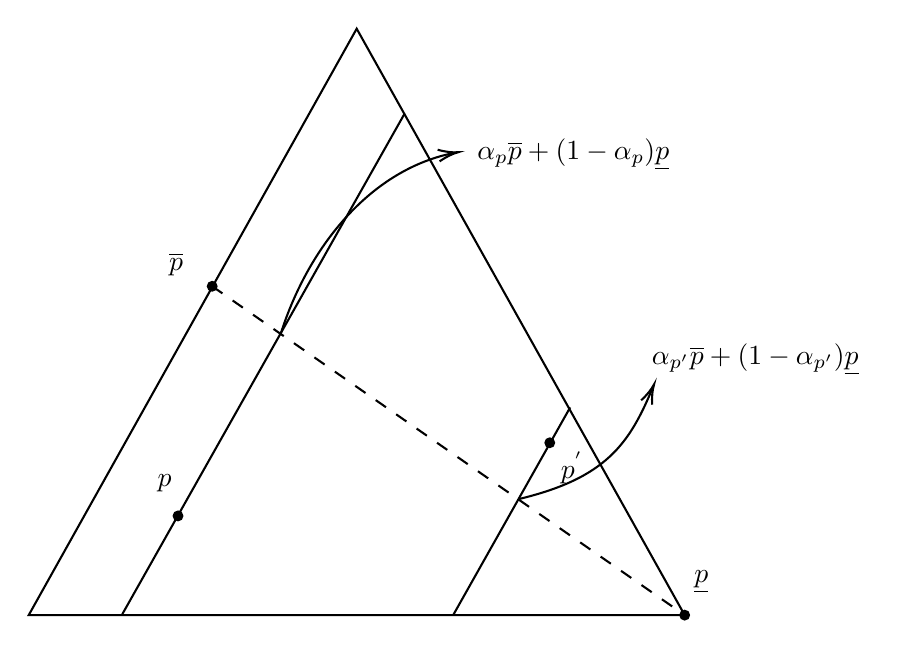
\begin{tikzpicture}[x=0.65pt,y=0.65pt,yscale=-1,xscale=1]
			%uncomment if require: \path (0,426); %set diagram left start at 0, and has height of 426

			%Shape: Triangle [id:dp8490740112879205] 
			\draw   (284.33,42.07) -- (466.67,368.07) -- (102,368.07) -- cycle ;
			%Shape: Circle [id:dp35031725224734067] 
			\draw  [fill={rgb, 255:red, 0; green, 0; blue, 0 }  ,fill opacity=1 ] (464.25,368.07) .. controls (464.25,366.74) and (465.33,365.66) .. (466.67,365.66) .. controls (468,365.66) and (469.08,366.74) .. (469.08,368.07) .. controls (469.08,369.41) and (468,370.49) .. (466.67,370.49) .. controls (465.33,370.49) and (464.25,369.41) .. (464.25,368.07) -- cycle ;
			%Shape: Circle [id:dp5994426130925808] 
			\draw  [fill={rgb, 255:red, 0; green, 0; blue, 0 }  ,fill opacity=1 ] (201.58,185.25) .. controls (201.58,183.92) and (202.67,182.83) .. (204,182.83) .. controls (205.33,182.83) and (206.42,183.92) .. (206.42,185.25) .. controls (206.42,186.58) and (205.33,187.67) .. (204,187.67) .. controls (202.67,187.67) and (201.58,186.58) .. (201.58,185.25) -- cycle ;
			%Straight Lines [id:da10409961384235067] 
			\draw  [dash pattern={on 4.5pt off 4.5pt}]  (204,185.25) -- (466.67,368.07) ;
			%Shape: Circle [id:dp20798560554542445] 
			\draw  [fill={rgb, 255:red, 0; green, 0; blue, 0 }  ,fill opacity=1 ] (389.25,272.25) .. controls (389.25,270.92) and (390.33,269.83) .. (391.67,269.83) .. controls (393,269.83) and (394.08,270.92) .. (394.08,272.25) .. controls (394.08,273.58) and (393,274.67) .. (391.67,274.67) .. controls (390.33,274.67) and (389.25,273.58) .. (389.25,272.25) -- cycle ;
			%Shape: Circle [id:dp4192734085033405] 
			\draw  [fill={rgb, 255:red, 0; green, 0; blue, 0 }  ,fill opacity=1 ] (182.58,312.92) .. controls (182.58,311.58) and (183.67,310.5) .. (185,310.5) .. controls (186.33,310.5) and (187.42,311.58) .. (187.42,312.92) .. controls (187.42,314.25) and (186.33,315.33) .. (185,315.33) .. controls (183.67,315.33) and (182.58,314.25) .. (182.58,312.92) -- cycle ;
			%Straight Lines [id:da3902197637661603] 
			\draw    (154,367.6) -- (311,89.2) ;
			%Straight Lines [id:da7454732907488841] 
			\draw    (338,368) -- (403,252.6) ;
			%Curve Lines [id:da5696173015502568] 
			\draw    (242,211.92) .. controls (257.84,161.91) and (293.28,119.59) .. (339.27,110.99) ;
			\draw [shift={(340.67,110.74)}, rotate = 170.27] [color={rgb, 255:red, 0; green, 0; blue, 0 }  ][line width=0.75]    (10.93,-3.29) .. controls (6.95,-1.4) and (3.31,-0.3) .. (0,0) .. controls (3.31,0.3) and (6.95,1.4) .. (10.93,3.29)   ;
			%Curve Lines [id:da32978400124499274] 
			\draw    (374.33,303.58) .. controls (422.93,291.92) and (435.95,272.98) .. (449.07,241.2) ;
			\draw [shift={(449.67,239.74)}, rotate = 112.2] [color={rgb, 255:red, 0; green, 0; blue, 0 }  ][line width=0.75]    (10.93,-3.29) .. controls (6.95,-1.4) and (3.31,-0.3) .. (0,0) .. controls (3.31,0.3) and (6.95,1.4) .. (10.93,3.29)   ;

			% Text Node
			\draw (178.33,165.07) node [anchor=north west][inner sep=0.75pt]    {$\overline{p}$};
			% Text Node
			\draw (470.33,341.4) node [anchor=north west][inner sep=0.75pt]    {$\underline{p}$};
			% Text Node
			\draw (349.67,101.4) node [anchor=north west][inner sep=0.75pt]    {$\alpha _{p}\overline{p} +( 1-\alpha _{p})\underline{p} \ $};
			% Text Node
			\draw (172,288.4) node [anchor=north west][inner sep=0.75pt]    {$p$};
			% Text Node
			\draw (396.08,275.65) node [anchor=north west][inner sep=0.75pt]    {$p^{'}$};
			% Text Node
			\draw (446.67,215.4) node [anchor=north west][inner sep=0.75pt]    {$\alpha _{p'}\overline{p} +( 1-\alpha _{p'})\underline{p} \ $};


		\end{tikzpicture}
		\caption{Step 3.}
		\label{fig:step3}
	\end{figure}

	First, notice that if \( \alpha_p \) exists, it must be unique. Suppose there are two such numbers, \( \alpha_p \) and \( \alpha_p' \), with \( \alpha_p > \alpha_p' \). Then, by \textbf{Step 2}, \( \alpha_p \overline{p} + (1-\alpha_p)\,\underline{p} \succ \alpha_p' \overline{p} + (1-\alpha_p')\,\underline{p} \), contradicting indifference to \( p \).

	Now we need to show that such an \( \alpha_p \) exists. If \( \overline{p} \sim p \), then \( \alpha_p = 1 \) works; if \( \underline{p} \sim p \), then \( \alpha_p = 0 \) works. The interesting case is when \( \overline{p} \succ p \succ \underline{p} \).

	Define
	\begin{equation}\label{eq:astar}
		\alpha_p \;=\; \sup \bigl\{\,\alpha \in [0,1] : p \succsim \alpha \overline{p} + (1-\alpha)\,\underline{p}\,\bigr\}.
	\end{equation}
	Since \( \alpha = 0 \) belongs to this set, the supremum is well defined and the set is non-empty.

	We now establish two auxiliary claims. The first is
	\begin{equation}\label{eq:claim0}
		\text{If } 1 \ge \alpha > \alpha_p, \text{ then } \alpha \overline{p} + (1-\alpha)\,\underline{p} \succ p .
	\end{equation}

	Indeed, if \( p \succsim \alpha \overline{p} + (1-\alpha)\,\underline{p} \) held for such \(\alpha\), then \(\alpha_p\) would not satisfy Equation~\eqref{eq:astar}. Moreover,
	\begin{equation}\label{eq:claim1}
		\text{If } 0 \le \alpha < \alpha_p, \text{ then } p \succ \alpha \overline{p} + (1-\alpha)\,\underline{p}.
	\end{equation}

	The reasoning is as follows. By the definition of \( \alpha_p \), there exists some \(\alpha'\) such that \(\alpha < \alpha' \le \alpha_p\) and \( p \succsim \alpha' \overline{p} + (1-\alpha')\,\underline{p} \). Since \( \alpha < \alpha' \), \textbf{Step 2} implies that
	\[
		p \succ \alpha' \overline{p} + (1-\alpha')\,\underline{p} \succ \alpha \overline{p} + (1-\alpha)\,\underline{p}.
	\]

	Now, there are three possibilities to consider:
	\( \alpha_p \overline{p} + (1-\alpha_p)\,\underline{p} \succ p \),
	\( p \succ \alpha_p \overline{p} + (1-\alpha_p)\,\underline{p} \),
	or indifference between them.

	If \( \alpha_p \overline{p} + (1-\alpha_p)\,\underline{p} \succ p \), then by \usename{axn:continuity} there exists \(\beta \in (0,1)\) such that
	\[
		\beta \bigl(\alpha_p \overline{p} + (1-\alpha_p)\,\underline{p}\bigr) + (1-\beta)\,\underline{p} \succ p.
	\]
	Notice that
	\[
		\begin{aligned}
			\beta \bigl(\alpha_p \overline{p} + (1-\alpha_p)\,\underline{p}\bigr) + (1-\beta)\,\underline{p}
			 & = \beta \alpha_p\,\overline{p} + \beta (1-\alpha_p)\,\underline{p} + (1-\beta)\,\underline{p} \\
			 & = \beta \alpha_p\,\overline{p} + \bigl[\beta (1-\alpha_p) + (1-\beta)\bigr]\,\underline{p}    \\
			 & = \beta \alpha_p\,\overline{p} + \bigl(1-\beta \alpha_p\bigr)\,\underline{p}
			\;\succ\; p.
		\end{aligned}
	\]

	Since \( \beta \alpha_p < \alpha_p \), by Equation~\eqref{eq:claim1} we must have \( p \succ \beta \alpha_p\,\overline{p} + (1-\beta \alpha_p)\,\underline{p} \), which is a contradiction.

	If instead \( p \succ \alpha_p \overline{p} + (1-\alpha_p)\,\underline{p} \), then by \usename{axn:continuity} there exists \( \beta \in (0,1) \) such that
	\[
		\begin{aligned}
			p \  & \succ\ \beta \bigl(\alpha_p \overline{p} + (1-\alpha_p)\,\underline{p}\bigr) + (1-\beta)\,\overline{p} \\
			     & =\ \bigl[\beta \alpha_p + (1-\beta)\bigr]\,\overline{p} + \beta (1-\alpha_p)\,\underline{p}            \\
			     & =\ \bigl(1-\beta (1-\alpha_p)\bigr)\,\overline{p} + \beta (1-\alpha_p)\,\underline{p}.
		\end{aligned}
	\]
	Since \( 1 - \beta (1-\alpha_p) > \alpha_p \), by Equation~\eqref{eq:claim0} we must have
	\[
		\bigl(1-\beta (1-\alpha_p)\bigr)\,\overline{p} + \beta (1-\alpha_p)\,\underline{p} \succ p,
	\]
	which is again a contradiction.

	\paragraph{Step 4.} Define a utility function \( U : \Delta(X) \to \mathbb{R} \) that assigns to each lottery a number representing its utility, defined by \( U(p) = \alpha_p \). This function represents preferences \( \succsim \).

	Take two lotteries \( p \) and \( p' \). By \textbf{Step 3}, there exist unique \( \alpha_p \) and \( \alpha_{p'} \) such that
	\[
		p \sim \alpha_p \overline{p} + (1-\alpha_p)\,\underline{p},
		\quad
		p' \sim \alpha_{p'} \overline{p} + (1-\alpha_{p'})\,\underline{p}.
	\]
	Therefore,
	\[
		p \succsim p'
		\ \text{if and only if}\
		\alpha_p \overline{p} + (1-\alpha_p)\,\underline{p}
		\succsim
		\alpha_{p'} \overline{p} + (1-\alpha_{p'})\,\underline{p}.
	\]
	By \textbf{Step 2},
	\[
		\alpha_p \overline{p} + (1-\alpha_p)\,\underline{p}
		\succsim
		\alpha_{p'} \overline{p} + (1-\alpha_{p'})\,\underline{p}
		\ \text{if and only if}\
		\alpha_p \ge \alpha_{p'}.
	\]
	The last condition holds if and only if \( U(p) \ge U(p') \), which proves the claim.

	\paragraph{Step 5.} The function \( U \) is linear and therefore, by Exercise~\ref{ex:linear}, has the expected utility form.

	From the previous steps we know that, for any lottery \( p \), there is a unique number \( U(p) \in [0,1] \) such that
	\[
		p \sim U(p)\,\overline{p} + \bigl(1-U(p)\bigr)\,\underline{p},
		\qquad
		p' \sim U(p')\,\overline{p} + \bigl(1-U(p')\bigr)\,\underline{p}.
	\]

	Applying \usename{axn:independence}, we get
	\begin{align*}
		\beta p + (1-\beta)p'
		 & \sim \beta\!\left[U(p)\,\overline{p} + \bigl(1-U(p)\bigr)\,\underline{p}\right] + (1-\beta)p' \\
		 & \sim \beta\!\left[U(p)\,\overline{p} + \bigl(1-U(p)\bigr)\,\underline{p}\right]
		+ (1-\beta)\!\left[U(p')\,\overline{p} + \bigl(1-U(p')\bigr)\,\underline{p}\right]               \\
		 & = \bigl[\beta U(p) + (1-\beta)U(p')\bigr]\,\overline{p}
		+ \Bigl(1 - \bigl[\beta U(p) + (1-\beta)U(p')\bigr]\Bigr)\,\underline{p}.
	\end{align*}

	Let \(\gamma := \beta U(p) + (1-\beta)U(p')\).
	By \textbf{Step 4}, for the lottery \(\beta p + (1-\beta)p'\) there is a \emph{unique} number \(\gamma\) such that
	\(\beta p + (1-\beta)p' \sim \gamma\,\overline{p} + (1-\gamma)\,\underline{p}\).
	Therefore,
	\[
		U\!\left(\beta p + (1-\beta)p'\right)
		= \beta U(p) + (1-\beta)U(p').
	\]
\end{proof}

Recall that a functional representation of preferences need not be unique: multiple functions can represent the same preferences. However, for expected utility representations we have a very specific characterization of all possible representations, as stated in the following corollary.

\begin{corollary}\label{cor:uniq}
	Suppose \( U \) is an expected utility representation of \( \succsim \). Then \( \widetilde U \colon \Delta(X) \to \mathbb{R} \) is another expected utility representation of \( \succsim \) if and only if there exist \( \beta > 0 \) and \( \gamma \in \mathbb{R} \) such that
	\begin{equation}\label{eq:affine}
		\widetilde U(p) \;=\; \beta\,U(p) + \gamma \qquad \text{for all } p .
	\end{equation}
\end{corollary}

\begin{proof}
	First, suppose that Equation~\eqref{eq:affine} holds. Then \(\widetilde U\) is an expected utility representation of \(\succsim\). Assume \(\widetilde U = \beta U + \gamma\) with \(\beta > 0\). Then
	\[
		\widetilde U(p)
		\;=\;
		\beta \sum_{x} p(x) u(x) + \gamma
		\;=\;
		\sum_{x} p(x)\bigl[\beta u(x) + \gamma\bigr].
	\]
	Hence, \(\widetilde U\) has the expected utility form with \(\widetilde u(x) := \beta u(x) + \gamma\). Since \(\beta > 0\), it follows that
	\( p \succsim q \iff U(p) \ge U(q) \iff \widetilde U(p) \ge \widetilde U(q) \).

	Second, suppose that \( U \) and \(\widetilde U\) are both expected utility
	representations of the same \(\succsim\). Then they must be related by an affine transformation as in Equation~\eqref{eq:affine}. By Lemma~\ref{lem:max}, there exist \(\overline{p}, \underline{p} \) such that \(\overline{p} \succ \underline{p}\) and \(\overline{p} \succsim p \succsim \underline{p}\) for all \(p\). For any lottery \(p\), define \(\alpha_p \in [0,1]\) by
	\[
		U(p)
		\;=\;
		\alpha_p U(\overline{p}) + (1-\alpha_p) U(\underline{p}),
		\quad \text{so that} \quad
		\alpha_p
		\;=\;
		\frac{U(p) - U(\underline{p})}{U(\overline{p}) - U(\underline{p})}.
	\]

	Applying the same construction to \(\widetilde U\) and using the \emph{same} \(\alpha_p\) (since both functions represent the \emph{same} preferences), we obtain
	\[
		\widetilde U(p)
		\;=\;
		\alpha_p \widetilde U(\overline{p}) + (1-\alpha_p)\,\widetilde U(\underline{p})
		\;=\;
		\widetilde U(\underline{p})
		\;+\;
		\frac{\widetilde U(\overline{p}) - \widetilde U(\underline{p})}
		{U(\overline{p}) - U(\underline{p})}
		\bigl[U(p) - U(\underline{p})\bigr].
	\]
	Rearranging yields the affine relation
	\[
		\widetilde U(p)
		\;=\;
		\beta\,U(p) + \gamma
		\quad \text{for all } p,
	\]
	where
	\[
		\beta
		\;:=\;
		\frac{\widetilde U(\overline{p}) - \widetilde U(\underline{p})}
		{U(\overline{p}) - U(\underline{p})}
		\;>\; 0,
		\qquad
		\gamma
		\;:=\;
		\widetilde U(\underline{p}) - \beta\,U(\underline{p}).
	\]
	Positivity of \(\beta\) follows because \(\overline{p} \succ \underline{p}\) implies
	\( U(\overline{p}) > U(\underline{p}) \) and
	\( \widetilde U(\overline{p}) > \widetilde U(\underline{p}) \).
\end{proof}

In Exercise~\ref{ex:diff}, you are asked to elaborate on the significance of Corollary~\ref{cor:uniq} for interpreting utility numbers as \emph{cardinal} representations of preferences.

\paragraph{Things to read.} For a textbook treatment of the material covered in this lecture, see \citet[pp.~170–178]{mas-colellMicroeconomicTheory1995}. Theorem~\ref{thm:eu} is known as the \emph{von Neumann–Morgenstern representation theorem}, after \citet{vonneumannTheoryGamesEconomic2007}, and it has enormous historical importance. An excellent discussion of the historical context and significance of expected utility theory can be found in \citet{moscatiMeasuringUtilityMarginal2018}.

\section{Exercises}

\begin{exercise}\label{ex:parallel-lines}
	Show that if preferences are represented by an expected utility function, then indifference curves in the triangle are parallel lines.
\end{exercise}

\begin{exercise}\label{ex:indlin}
	Explain why the fact that indifference curves are straight and parallel lines follows from \usename{axn:independence}.
\end{exercise}

\begin{exercise}
	Prove the direction of Theorem~\ref{thm:eu} that we did not prove in class. Show that if \( U \) represents \( \succsim \), then \( \succsim \) satisfies \usename{axn:wo}, \usename{axn:continuity}, and \usename{axn:independence}. (It is not difficult, I promise!)
\end{exercise}

\begin{exercise}
	Revisit the choice problem in Exercise~\ref{ex:allais}. Show that the preferences exhibited there do not satisfy \usename{axn:independence}.
\end{exercise}

\begin{exercise}
	Consider the \textbf{Betweenness Axiom} introduced by \citet{dekelAxiomaticCharacterizationPreferences1986}: for all lotteries \( p, q \) and \( \alpha \in [0,1] \), if \( p \sim q \), then \( \alpha p + (1-\alpha) q \sim p \). Show that \usename{axn:independence} implies Betweenness, but Betweenness does not imply \usename{axn:independence}. (Hint: for the second part, construct a preference relation that satisfies Betweenness but not \usename{axn:independence}.) Are indifference curves still linear under Betweenness? Are they parallel?
\end{exercise}

\begin{exercise}
	Show that the choices of the individual in Exercise~\ref{ex:allais} are compatible with Betweenness. (Hint: drawing a picture might help.)
\end{exercise}

\begin{exercise}\label{ex:diff}
	Explain why Corollary~\ref{cor:uniq} allows us to make statements such as \textquote{the utility of winning the lottery is twice the utility of not winning.}
\end{exercise}

\begin{comment}

\begin{solution}[ex:parallel-lines]
	Let \(\{x,y,z\}\) be the outcomes and let

	\[ U(p)=\sum_{w\in\{x,y,z\}} u(w)\,p(w) \]

	be the expected utility
	of lottery \(p\). Since \(p(z)=1-p(x)-p(y)\), we can write
	\[
		U(p) \;=\; \big(u(x)-u(z)\big)\,p(x)\;+\;\big(u(y)-u(z)\big)\,p(y)\;+\;u(z).
	\]

	Fix a utility level \(c\). The indifference set \(\{p:U(p)=c\}\) satisfies
	\[
		\big(u(x)-u(z)\big)\,p(x)\;+\;\big(u(y)-u(z)\big)\,p(y)\;=\;c-u(z).
	\]

	Solving for \(p(y)\) as a function of \(p(x)\),
	\[
		p(y)\;=\;\frac{c-u(z)}{\,u(y)-u(z)\,}\;-\;\frac{u(x)-u(z)}{\,u(y)-u(z)\,}\,p(x).
	\]

	The coefficient of \(p(x)\) is
	\[
		-\frac{u(x)-u(z)}{\,u(y)-u(z)\,},
	\]
	which does not depend on \(c\). Changing \(c\) only changes the intercept
	\(\frac{c-u(z)}{u(y)-u(z)}\). Therefore, all indifference lines, the portions of these lines that lie inside the simplex, have the same slope and are parallel.
\end{solution}

\end{comment}

\bibliographystyle{apacite}  % or another  style
\bibliography{references} % .bib file goes in ./bib/